\subsubsection{UC26 - Accesso alla merchant dashboard}
\begin{itemize}
\item \textbf{Attori primari}: venditore;
\item \textbf{Descrizione}: il venditore accede alla merchant dashboard\ped{G};
\item \textbf{Scenario Principale}: il venditore, tramite l'apposito pulsante, accede alla merchant dashboard\ped{G};
\item \textbf{Precondizione}: il venditore ha effettuato l'autenticazione ed è stato riconosciuto come venditore;
\item \textbf{Postcondizione}: il venditore si trova nella merchant dashboard\ped{G};
\end{itemize}

\subsubsection{UC27 - Inserimento prodotto}
\begin{itemize}
\item \textbf{Attori primari}: venditore;
\item \textbf{Descrizione}: il venditore può inserire nel sistema nuovi prodotti da vendere;
\item \textbf{Scenario Principale}: il venditore accede alla pagina di inserimento prodotti tramite l'apposito pulsante ed inserisce le seguenti informazioni:
\begin{itemize}
	\item nome \textbf{[UC27.1]};
	\item descrizione \textbf{[UC27.2]};
	\item prezzo \textbf{[UC27.3]};
	\item immagine \textbf{[UC27.4]};
	\item categoria \textbf{[UC27.5]}.
\end{itemize}
In seguito verrà premuto il pulsante di conferma \textbf{[UC27.6]};
\item \textbf{Precondizione}: l'utente ha eseguito il login, è riconosciuto come venditore e si trova nella merchant dashboard\ped{G};
\item \textbf{Postcondizione}: il venditore ha inserito un nuovo prodotto nel sistema.
\end{itemize}

\begin{figure}[H]
\centering
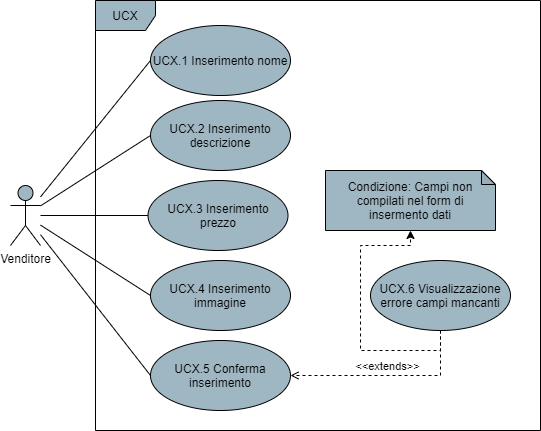
\includegraphics[scale=0.6]{res/UseCase/Immagini/InserimentoProdotto}
\caption{Diagramma UML\ped{G} per UC27 - Inserimento prodotto}
\end{figure}

\subsubsection{UC27.1 - Inserimento nome}
\begin{itemize}
\item \textbf{Attori primari}: venditore;
\item \textbf{Descrizione}: al venditore è richiesto l'inserimento del nome del nuovo prodotto da inserire;
\item \textbf{Scenario Principale}: il venditore inserisce nel form dedicato il nome del nuovo prodotto;
\item \textbf{Precondizione}: il venditore si trova nella pagina dedicata all'inserimento di un nuovo prodotto;
\item \textbf{Postcondizione}: il venditore ha compilato il campo dedicato al nome del prodotto.
\end{itemize}

\subsubsection{UC27.2 - Inserimento descrizione}
\begin{itemize}
\item \textbf{Attori primari}: venditore;
\item \textbf{Descrizione}: al venditore è richiesto l'inserimento della descrizione del nuovo prodotto da inserire;
\item \textbf{Scenario Principale}: il venditore inserisce nel form dedicato la descrizione del nuovo prodotto;
\item \textbf{Precondizione}: il venditore si trova nella pagina dedicata all'inserimento di un nuovo prodotto;
\item \textbf{Postcondizione}: il venditore ha compilato il campo dedicato alla descrizione del prodotto.
\end{itemize}

\subsubsection{UC27.3 - Inserimento prezzo}
\begin{itemize}
\item \textbf{Attori primari}: venditore;
\item \textbf{Descrizione}: al venditore è richiesto l'inserimento del prezzo del nuovo prodotto da inserire;
\item \textbf{Scenario Principale}: il venditore inserisce nel form dedicato il prezzo del nuovo prodotto;
\item \textbf{Precondizione}: il venditore si trova nella pagina dedicata all'inserimento di un nuovo prodotto;
\item \textbf{Postcondizione}: il venditore ha compilato il campo dedicato al prezzo del prodotto.
\end{itemize}

\subsubsection{UC27.4 - Inserimento immagine}
\begin{itemize}
\item \textbf{Attori primari}: venditore;
\item \textbf{Descrizione}: al venditore è richiesto l'inserimento dell'immagine del nuovo prodotto da inserire;
\item \textbf{Scenario Principale}: il venditore carica tramite l'apposito bottone di upload l'immagine del nuovo prodotto;
\item \textbf{Precondizione}: il venditore si trova nella pagina dedicata all'inserimento di un nuovo prodotto;
\item \textbf{Postcondizione}: il venditore ha caricato l'immagine del nuovo prodotto.
\end{itemize}

\subsubsection{UC27.5 - Inserimento categoria}
\begin{itemize}
\item \textbf{Attori primari}: venditore;
\item \textbf{Descrizione}: al venditore è richiesto l'inserimento della categoria del nuovo prodotto da inserire;
\item \textbf{Scenario Principale}: il venditore inserisce nel form dedicato la categoria del nuovo prodotto;
\item \textbf{Precondizione}: il venditore si trova nella pagina dedicata all'inserimento di un nuovo prodotto;
\item \textbf{Postcondizione}: il venditore ha compilato il campo dedicato alla categoria del prodotto.
\end{itemize}

\subsubsection{UC27.6 - Conferma inserimento}
\begin{itemize}
\item \textbf{Attori primari}: venditore;
\item \textbf{Descrizione}: il venditore conferma i dati presenti nel form e inserisce il nuovo prodotto;
\item \textbf{Scenario Principale}: il venditore preme il pulsante di conferma e inserisce il nuovo prodotto con i dati precedentemente inseriti;
\item \textbf{Estensioni}: 
\begin{itemize}
\item nel caso qualche campo non sia compilato viene visualizzato un messaggio di errore \textbf{[UC27.7]}.
\end{itemize} 
\item \textbf{Precondizione}: il venditore si trova nella pagina dedicata all'inserimento di un nuovo prodotto e ha premuto il bottone di conferma;
\item \textbf{Postcondizione}: il venditore ha inserito un nuovo prodotto nel sistema.
\end{itemize}

\subsubsection{UC27.7 - Visualizzazione errore campi mancanti inserimento prodotto}
\begin{itemize}
\item \textbf{Attori primari}: venditore;
\item \textbf{Descrizione}: il venditore visualizza un messaggio di errore che lo informa che per procedere all'inserimento è necessario aver inserito tutti i dati richiesti;
\item \textbf{Scenario Principale}: il venditore prova ad inserire un nuovo prodotto senza aver compilato tutti i campi dati;
\item \textbf{Precondizione}: il venditore si trova nella pagina dedicata all'inserimento di un nuovo prodotto, ha premuto il bottone di conferma e non sono stati compilati tutti i campi;
\item \textbf{Postcondizione}: viene visualizzato un messaggio che informa il venditore della necessità di compilare tutti i campi dati per completare l'inserimento di un prodotto.
\end{itemize}

\subsubsection{UC28 - Visualizzazione lista prodotti}
\begin{itemize}
\item \textbf{Attori primari}: venditore;
\item \textbf{Descrizione}: il venditore visualizza nella merchant dashboard\ped{G} la lista dei prodotti presenti nel sistema;
\item \textbf{Scenario Principale}: il venditore accede alla merchant dashboard\ped{G} e, nell'apposita sezione, visualizza le seguenti informazioni sui prodotti nel sistema:
\begin{itemize}
\item nome;
\item descrizione;
\item categoria;
\item prezzo;
\item immagine.
\end{itemize}
\item \textbf{Precondizione}: l'utente ha eseguito il login, è riconosciuto come venditore e si trova nella merchant dashboard\ped{G};
\item \textbf{Postcondizione}: il venditore visualizza la lista dei prodotti presenti nel sistema, ognuno dei quali con le seguenti informazioni:
\begin{itemize}
\item nome;
\item descrizione;
\item categoria;
\item prezzo;
\item immagine.
\end{itemize}
\end{itemize}

\subsubsection{UC29 - Modifica prodotto}
\begin{itemize}
\item \textbf{Attori primari}: venditore;
\item \textbf{Descrizione}: il venditore può modificare i prodotti presenti nel sistema;
\item \textbf{Scenario Principale}: il venditore accede alla pagina di modifica tramite l'apposito pulsante collegato al prodotto da modificare, visualizzato nella lista dei prodotti \textbf{[UC28]}. Da li può modificare le seguenti informazioni:
\begin{itemize}
	\item nome \textbf{[UC29.1]};
	\item descrizione \textbf{[UC29.2]};
	\item prezzo \textbf{[UC29.3]};
	\item immagine \textbf{[UC29.4]};
	\item categoria \textbf{[UC29.5]}.
\end{itemize}
In seguito verrà premuto il pulsante di conferma \textbf{[UC29.6]};
\item \textbf{Precondizione}: l'utente ha eseguito il login, è riconosciuto come venditore e si trova nella merchant dashboard\ped{G};
\item \textbf{Postcondizione}: il venditore ha modificato il prodotto selezionato.
\end{itemize}

\begin{figure}[H]
\centering
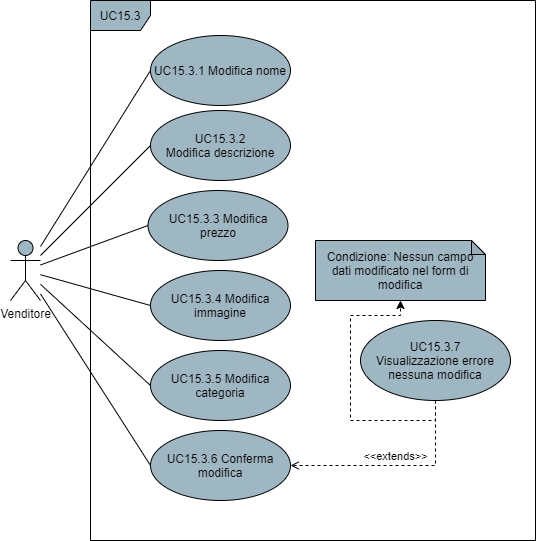
\includegraphics[scale=0.6]{res/UseCase/Immagini/ModificaProdotto}
\caption{Diagramma UML\ped{G} per UC29 - Modifica prodotto}
\end{figure}

\subsubsection{UC29.1 - Modifica nome}
\begin{itemize}
\item \textbf{Attori primari}: venditore;
\item \textbf{Descrizione}: il venditore modifica il nome del prodotto selezionato;
\item \textbf{Scenario Principale}: il venditore visualizza nel campo relativo al nome del prodotto il dato attualmente presente, che andrà a sovrascrivere con il nuovo nome aggiornato;
\item \textbf{Precondizione}: il venditore si trova nella pagina dedicata alla modifica di un prodotto;
\item \textbf{Postcondizione}: il venditore ha compilato il campo dedicato al nome del prodotto, sovrascrivendo il precedente.
\end{itemize}

\subsubsection{UC29.2 - Modifica descrizione}
\begin{itemize}
\item \textbf{Attori primari}: venditore;
\item \textbf{Descrizione}: il venditore modifica la descrizione del prodotto selezionato;
\item \textbf{Scenario Principale}: il venditore visualizza nel campo relativo alla descrizione del prodotto il dato attualmente presente, che andrà a sovrascrivere con la nuova descrizione aggiornata;
\item \textbf{Precondizione}: il venditore si trova nella pagina dedicata alla modifica di un prodotto;
\item \textbf{Postcondizione}: il venditore ha compilato il campo dedicato alla descrizione del prodotto, sovrascrivendo la precedente.
\end{itemize}

\subsubsection{UC29.3 - Modifica prezzo}
\begin{itemize}
\item \textbf{Attori primari}: venditore;
\item \textbf{Descrizione}: il venditore modifica il prezzo del prodotto selezionato;
\item \textbf{Scenario Principale}: il venditore visualizza nel campo relativo al prezzo del prodotto il dato attualmente presente, che andrà a sovrascrivere con il nuovo prezzo aggiornato;
\item \textbf{Precondizione}: il venditore si trova nella pagina dedicata alla modifica di un prodotto;
\item \textbf{Postcondizione}: il venditore ha compilato il campo dedicato al prezzo del prodotto, sovrascrivendo il precedente.
\end{itemize}

\subsubsection{UC29.4 - Modifica immagine}
\begin{itemize}
\item \textbf{Attori primari}: venditore;
\item \textbf{Descrizione}: il venditore modifica l'immagine del prodotto selezionato;
\item \textbf{Scenario Principale}: il venditore visualizza nel campo relativo all'immagine del prodotto quella attualmente presente, che andrà a sovrascrivere caricando la nuova immagine aggiornata;
\item \textbf{Precondizione}: il venditore si trova nella pagina dedicata alla modifica di un prodotto;
\item \textbf{Postcondizione}: il venditore ha caricato l'immagine del prodotto, sovrascrivendo la precedente.
\end{itemize}

\subsubsection{UC29.5 - Modifica categoria}
\begin{itemize}
\item \textbf{Attori primari}: venditore;
\item \textbf{Descrizione}: il venditore modifica la categoria del prodotto selezionato;
\item \textbf{Scenario Principale}: il venditore visualizza nel campo relativo alla categoria del prodotto il dato attualmente presente, che andrà a sovrascrivere con la nuova categoria aggiornata;
\item \textbf{Precondizione}: il venditore si trova nella pagina dedicata alla modifica di un prodotto;
\item \textbf{Postcondizione}: il venditore ha compilato il campo dedicato alla categoria del prodotto, sovrascrivendo la precedente.
\end{itemize}

\subsubsection{UC29.6 - Conferma modifica}
\begin{itemize}
\item \textbf{Attori primari}: venditore;
\item \textbf{Descrizione}: il venditore conferma i dati presenti nel form e modifica il prodotto;
\item \textbf{Scenario Principale}: il venditore preme il pulsante di conferma e modifica il prodotto selezionato con i dati precedentemente inseriti;
\item \textbf{Estensioni}: 
\begin{itemize}
	\item se non viene sovrascritto nessun dato viene visualizzato un messaggio di errore \textbf{[UC29.7]}.
\end{itemize} 
\item \textbf{Precondizione}: il venditore si trova nella pagina dedicata alla modifica di un prodotto e ha premuto il bottone di conferma;
\item \textbf{Postcondizione}: il venditore ha modificato il prodotto selezionato.
\end{itemize}

\subsubsection{UC29.7 - Visualizzazione errore nessuna modifica}
\begin{itemize}
\item \textbf{Attori primari}: venditore;
\item \textbf{Descrizione}: il venditore visualizza un messaggio di errore che lo informa che per procedere alla modifica è necessario aver sovrascritto almeno un campo dati;
\item \textbf{Scenario Principale}: il venditore prova a modificare un nuovo prodotto senza aver sovrascritto almeno un campo dati;
\item \textbf{Precondizione}: il venditore si trova nella pagina dedicata alla modifica di un prodotto e ha premuto il bottone di conferma;
\item \textbf{Postcondizione}: viene visualizzato un messaggio che informa il venditore della necessità di compilare tutti i campi dati per completare la modifica di un prodotto.
\end{itemize}

\subsubsection{UC30 - Rimozione prodotto}
\begin{itemize}
\item \textbf{Attori primari}: venditore;
\item \textbf{Descrizione}: il venditore può rimuovere i prodotti presenti nel sistema;
\item \textbf{Scenario Principale}: il venditore elimina il prodotto scelto tramite l'apposito pulsante collegato al prodotto da eliminare, visualizzato nella lista dei prodotti \textbf{[UC28]};
\item \textbf{Precondizione}: l'utente ha eseguito il login, è riconosciuto come venditore e si trova nella merchant dashboard\ped{G};
\item \textbf{Postcondizione}: il venditore ha eliminato il prodotto selezionato.
\end{itemize}

\subsubsection{UC31 - Visualizzazione lista categorie}
\begin{itemize}
\item \textbf{Attori primari}: venditore;
\item \textbf{Descrizione}: il venditore visualizza nella merchant dashboard\ped{G} la lista delle categorie presenti nel sistema;
\item \textbf{Scenario Principale}: il venditore accede alla merchant dashboard\ped{G} e, nell'apposita sezione, visualizza la lista dei nomi delle categorie presenti;
\item \textbf{Precondizione}: l'utente ha eseguito il login, è riconosciuto come venditore e si trova nella merchant dashboard\ped{G};
\item \textbf{Postcondizione}: il venditore visualizza la lista dei nomi delle categorie presenti nel sistema.
\end{itemize}

\subsubsection{UC32 - Inserimento categoria}
\begin{itemize}
\item \textbf{Attori primari}: venditore;
\item \textbf{Descrizione}: il venditore può inserire nel sistema nuove categorie di prodotti;
\item \textbf{Scenario Principale}: il venditore accede alla pagina di inserimento categorie tramite l'apposito pulsante ed inserisce il nome della categoria \textbf{[UC32.1]} per poi premere il pulsante di conferma \textbf{[UC32.2]};
\item \textbf{Precondizione}: l'utente ha eseguito il login, è riconosciuto come venditore e si trova nella merchant dashboard\ped{G};
\item \textbf{Postcondizione}: il venditore ha inserito una nuova categoria nel sistema.
\end{itemize}

\begin{figure}[H]
\centering
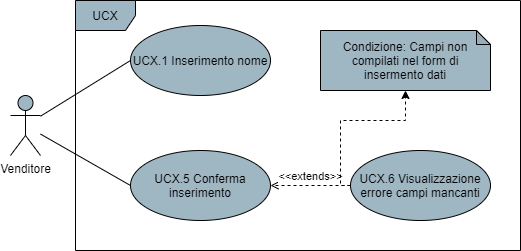
\includegraphics[scale=0.6]{res/UseCase/Immagini/InserimentoCategoria}
\caption{Diagramma UML\ped{G} per UC32 - Inserimento categoria}
\end{figure}

\subsubsection{UC32.1 - Inserimento nome}
\begin{itemize}
\item \textbf{Attori primari}: venditore;
\item \textbf{Descrizione}: al venditore è richiesto l'inserimento del nome della nuova categoria da inserire;
\item \textbf{Scenario Principale}: il venditore inserisce nel form dedicato il nome della nuova categoria;
\item \textbf{Precondizione}: il venditore si trova nella pagina dedicata all'inserimento di una nuova categoria;
\item \textbf{Postcondizione}: il venditore ha compilato il campo dedicato al nome della categoria.
\end{itemize}

\subsubsection{UC32.2 - Conferma inserimento}
\begin{itemize}
\item \textbf{Attori primari}: venditore;
\item \textbf{Descrizione}: il venditore conferma i dati presenti nel form e inserisce la nuova categoria;
\item \textbf{Scenario Principale}: il venditore preme il pulsante di conferma e inserisce la nuova categoria con il nome precedentemente inserito;
\item \textbf{Estensioni}: 
\begin{itemize}
	\item se il nome della categoria non è stato inserito o la categoria è già presente viene visualizzato un messaggio di errore \textbf{[UC32.3]}.
\end{itemize} 
\item \textbf{Precondizione}: il venditore si trova nella pagina dedicata all'inserimento di una nuova categoria e ha premuto il bottone di conferma;
\item \textbf{Postcondizione}: il venditore ha inserito una nuova categoria nel sistema.
\end{itemize}

\subsubsection{UC32.3 - Visualizzazione errore categoria inserita non valida}
\begin{itemize}
\item \textbf{Attori primari}: venditore;
\item \textbf{Descrizione}: il venditore visualizza un messaggio di errore che lo informa che per procedere all'inserimento è necessario aver inserito il nome di una categoria valida;
\item \textbf{Scenario Principale}: il venditore prova ad inserire una nuova categoria senza aver compilato il campo dati del nome o inserendo una categoria già esistente;
\item \textbf{Precondizione}: il venditore si trova nella pagina dedicata all'inserimento di una nuova categoria e ha premuto il bottone di conferma;
\item \textbf{Postcondizione}: viene visualizzato un messaggio che informa il venditore della necessità di compilare il campo del nome per inserire una nuova categoria o di inserire un nome non già esistente.
\end{itemize}

\subsubsection{UC33 - Rimozione categoria}
\begin{itemize}
\item \textbf{Attori primari}: venditore;
\item \textbf{Descrizione}: il venditore può rimuovere le categorie;
\item \textbf{Scenario Principale}: il venditore elimina la categoria scelta tramite l'apposito pulsante collegato alla categoria da eliminare, visualizzato nella lista delle categorie \textbf{[UC31]};
\item \textbf{Precondizione}: l'utente ha eseguito il login, è riconosciuto come venditore e si trova nella merchant dashboard\ped{G};
\item \textbf{Postcondizione}: il venditore ha eliminato la categoria selezionata.
\end{itemize}


\subsubsection{UC34 - Visualizzazione lista ordini}
\begin{itemize}
\item \textbf{Attori primari}: venditore;
\item \textbf{Descrizione}: il venditore visualizza nella merchant dashboard\ped{G} la lista degli ordini ricevuti;
\item \textbf{Scenario Principale}: il venditore accede alla merchant dashboard\ped{G} e, nell'apposita sezione, visualizza una lista degli ordini ricevuti. Per ogni ordine viene visualizzato il numero dell'ordine, il costo totale e la data. Il venditore può accedere ad altre informazioni premendo il bottone 'Dettagli' collegato all'ordine interessato \textbf{[UC34.1]};
\item \textbf{Precondizione}: l'utente ha eseguito il login, è riconosciuto come venditore e si trova nella merchant dashboard\ped{G};
\item \textbf{Postcondizione}: il venditore visualizza la lista degli ordini presenti nel sistema.
\end{itemize}

\begin{figure}[H]
\centering
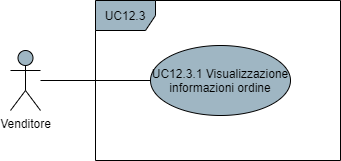
\includegraphics[scale=0.6]{res/UseCase/Immagini/VisualizzazioneOrdiniMerchant}
\caption{Diagramma UML\ped{G} per UC34 - Visualizzazione lista ordini ricevuti}
\end{figure}

\subsubsection{UC34.1 - Visualizzazione informazioni ordine}
\begin{itemize}
\item \textbf{Attori primari}: venditore;
\item \textbf{Descrizione}: il venditore visualizza le informazioni dell'ordine selezionato;
\item \textbf{Scenario Principale}: il venditore accede alla pagina di visualizzazione informazioni ordine tramite il pulsante 'Dettagli' collegato all'ordine selezionato nella lista degli ordini ricevuti \textbf{[UC34]}. In particolare vengono visualizzati i seguenti dati:
\begin{itemize}
	\item numero ordine;
	\item prodotti acquistati;
	\item quantità prodotti acquistati;
	\item costo per singola voce;
	\item costo totale;
	\item tasse applicate;
	\item data acquisto.
\end{itemize}
\item \textbf{Precondizione}: l'utente ha eseguito il login, è riconosciuto come venditore e si trova nella merchant dashboard\ped{G};
\item \textbf{Postcondizione}: il venditore visualizza le informazioni relative all'ordine selezionato.
\end{itemize}

\subsubsection{UC35 - Visualizzazione collegamenti a sistemi di gestione}
\begin{itemize}
\item \textbf{Attori primari}: venditore;
\item \textbf{Descrizione}: il venditore visualizza nella merchant dashboard\ped{G} i collegamenti agli strumenti di gestione esterni;
\item \textbf{Scenario Principale}: il venditore accede alla merchant dashboard\ped{G} e, nell'apposita sezione, visualizza dei collegamenti alla piattaforma di monitoraggio dell'applicazione e agli strumenti di configurazione;
\item \textbf{Precondizione}: l'utente ha eseguito il login, è riconosciuto come venditore e si trova nella merchant dashboard\ped{G};
\item \textbf{Postcondizione}: il venditore visualizza la lista dei collegamenti ai sistemi di gestione del sito.
\end{itemize}